\documentclass[11pt,letterpaper]{article}
\usepackage[utf8]{inputenc}
\usepackage[left=1in,right=1in,top=1in,bottom=1in]{geometry}
\usepackage{amsfonts,amsmath}
\usepackage{graphicx,float}
% -----------------------------------
\usepackage{hyperref}
\hypersetup{%
  colorlinks=true,
  linkcolor=blue,
  citecolor=blue,
  urlcolor=blue,
  linkbordercolor={0 0 1}
}
% -----------------------------------
\usepackage[style=authoryear-icomp,backend=biber]{biblatex}
\addbibresource{citation.bib}
% -----------------------------------
\usepackage{fancyhdr}
\newcommand\course{MATH-UA.0252\\Numerical Analysis}
\newcommand\hwnumber{5}                  % <-- homework number
\newcommand\NetIDa{Ryan Sh\`iji\'e D\`u} 
\newcommand\NetIDb{October 13th, 2023}
\pagestyle{fancyplain}
\headheight 35pt
\lhead{\NetIDa\\\NetIDb}
\chead{\textbf{\Large Worksheet \hwnumber}}
\rhead{\course}
\lfoot{}
\cfoot{}
\rfoot{\small\thepage}
\headsep 1.5em
% -----------------------------------
\usepackage{titlesec}
\renewcommand\thesubsection{(\arabic{section}.\alph{subsection})}
\titleformat{\subsection}[runin]
        {\normalfont\bfseries}
        {\thesubsection}% the label and number
        {0.5em}% space between label/number and subsection title
        {}% formatting commands applied just to subsection title
        []% punctuation or other commands following subsection title
% -----------------------------------
\setlength{\parindent}{0.0in}
\setlength{\parskip}{0.1in}
% -----------------------------------
\newcommand{\de}{\mathrm{d}}
\newcommand{\DD}{\mathrm{D}}
\newcommand{\pe}{\partial}
\newcommand{\mcal}{\mathcal}
%\newcommand{\pdx}{\left|\frac{\partial}{\partial_x}\right|}

\newcommand{\dsp}{\displaystyle}

\newcommand{\norm}[1]{\left\Vert #1 \right\Vert}
%\newcommand{\mean}[1]{\left\langle #1 \right\rangle}
\newcommand{\mean}[1]{\overline{#1}}
\newcommand{\inner}[2]{\left\langle #1,#2\right\rangle}

\newcommand{\ve}[1]{\boldsymbol{#1}}

\newcommand{\thus}{\Rightarrow \quad }
\newcommand{\fff}{\iff\quad}
\newcommand{\qdt}[1]{\quad \mbox{#1} \quad}

\renewcommand{\Re}{\mathrm{Re}}
\renewcommand{\Im}{\mathrm{Im}}
\newcommand{\E}{\mathbb{E}}
\newcommand{\lap} {\nabla^2}
\renewcommand{\div}{\nabla\cdot}

\newcommand{\csch}{\text{csch}}
\newcommand{\sech}{\text{sech}}


\newcommand{\hot}{\text{h.o.t.}}

\newcommand{\ssp}{\left.\qquad\right.}

\newcommand{\var}{\text{var}}
\newcommand{\cov}{\text{cov}}

%%%%%%%%%%%%%%%%%%%%%%%%%%%%%%%%%%%%%%%%%%%%%%%%%%
\makeatletter
\newcommand*{\mint}[1]{%
  % #1: overlay symbol
  \mint@l{#1}{}%
}
\newcommand*{\mint@l}[2]{%
  % #1: overlay symbol
  % #2: limits
  \@ifnextchar\limits{%
    \mint@l{#1}%
  }{%
    \@ifnextchar\nolimits{%
      \mint@l{#1}%
    }{%
      \@ifnextchar\displaylimits{%
        \mint@l{#1}%
      }{%
        \mint@s{#2}{#1}%
      }%
    }%
  }%
}
\newcommand*{\mint@s}[2]{%
  % #1: limits
  % #2: overlay symbol
  \@ifnextchar_{%
    \mint@sub{#1}{#2}%
  }{%
    \@ifnextchar^{%
      \mint@sup{#1}{#2}%
    }{%
      \mint@{#1}{#2}{}{}%
    }%
  }%
}
\def\mint@sub#1#2_#3{%
  \@ifnextchar^{%
    \mint@sub@sup{#1}{#2}{#3}%
  }{%
    \mint@{#1}{#2}{#3}{}%
  }%
}
\def\mint@sup#1#2^#3{%
  \@ifnextchar_{%
    \mint@sup@sub{#1}{#2}{#3}%
  }{%
    \mint@{#1}{#2}{}{#3}%
  }%
}
\def\mint@sub@sup#1#2#3^#4{%
  \mint@{#1}{#2}{#3}{#4}%
}
\def\mint@sup@sub#1#2#3_#4{%
  \mint@{#1}{#2}{#4}{#3}%
}
\newcommand*{\mint@}[4]{%
  % #1: \limits, \nolimits, \displaylimits
  % #2: overlay symbol: -, =, ...
  % #3: subscript
  % #4: superscript
  \mathop{}%
  \mkern-\thinmuskip
  \mathchoice{%
    \mint@@{#1}{#2}{#3}{#4}%
        \displaystyle\textstyle\scriptstyle
  }{%
    \mint@@{#1}{#2}{#3}{#4}%
        \textstyle\scriptstyle\scriptstyle
  }{%
    \mint@@{#1}{#2}{#3}{#4}%
        \scriptstyle\scriptscriptstyle\scriptscriptstyle
  }{%
    \mint@@{#1}{#2}{#3}{#4}%
        \scriptscriptstyle\scriptscriptstyle\scriptscriptstyle
  }%
  \mkern-\thinmuskip
  \int#1%
  \ifx\\#3\\\else_{#3}\fi
  \ifx\\#4\\\else^{#4}\fi  
}
\newcommand*{\mint@@}[7]{%
  % #1: limits
  % #2: overlay symbol
  % #3: subscript
  % #4: superscript
  % #5: math style
  % #6: math style for overlay symbol
  % #7: math style for subscript/superscript
  \begingroup
    \sbox0{$#5\int\m@th$}%
    \sbox2{$#5\int_{}\m@th$}%
    \dimen2=\wd0 %
    % => \dimen2 = width of \int
    \let\mint@limits=#1\relax
    \ifx\mint@limits\relax
      \sbox4{$#5\int_{\kern1sp}^{\kern1sp}\m@th$}%
      \ifdim\wd4>\wd2 %
        \let\mint@limits=\nolimits
      \else
        \let\mint@limits=\limits
      \fi
    \fi
    \ifx\mint@limits\displaylimits
      \ifx#5\displaystyle
        \let\mint@limits=\limits
      \fi
    \fi
    \ifx\mint@limits\limits
      \sbox0{$#7#3\m@th$}%
      \sbox2{$#7#4\m@th$}%
      \ifdim\wd0>\dimen2 %
        \dimen2=\wd0 %
      \fi
      \ifdim\wd2>\dimen2 %
        \dimen2=\wd2 %
      \fi
    \fi
    \rlap{%
      $#5%
        \vcenter{%
          \hbox to\dimen2{%
            \hss
            $#6{#2}\m@th$%
            \hss
          }%
        }%
      $%
    }%
  \endgroup
}

\begin{document} 

\section{Condition numbers and pivoted LU}
\subsection{}
Solve the matrix equation $\ve A\ve x = \ve b$ with 
\begin{align*}
  \ve A:=
  \begin{bmatrix}
    1       & 0  \\
    10^{4}  & 1
  \end{bmatrix}
  \qdt{ and }
  \ve b = \begin{bmatrix}
  0\\1
  \end{bmatrix}.
\end{align*}
What is $\kappa_\infty(A)$?

Consider a small perturbation $\Delta \ve b=[10^{-3},0]^\top$ being added to the right-hand side, and solve again. Repeat with $\Delta \ve b =[0,10^{-3}]^\top$. You should see that small perturbation can, but does not have to have a large effect even for badly conditioned systems.

\subsection{}
Verify the following LU decomposition of a matrix $A$ without pivoting:
  $$
  \ve A := \begin{bmatrix} 10^{-4} & 1\\ 1 & 1
  \end{bmatrix} = \ve L\ve U =
  \begin{bmatrix} 1 & 0\\ 10^4 & 1
  \end{bmatrix}
  \begin{bmatrix} 10^{-4} & 1\\ 0 & 1-10^4
  \end{bmatrix}
  $$ 
We have seen in the previous problem that solving a system with the matrix $\ve L$ is sensitive to errors, i.e., it is poorly conditioned. However, the original $\ve A$ matrix is well-conditioned.

Now the LU factorization of $\ve A$ with pivoting is
\begin{align*}
\ve P\ve A = \begin{bmatrix} 1 & 1 \\ 10^{-4} & 1
  \end{bmatrix} = \ve L\ve U =
  \begin{bmatrix} 1 & 0\\ 10^{-4} & 1
  \end{bmatrix}
  \begin{bmatrix} 1 & 1\\ 0 & 1-10^{-4}
  \end{bmatrix}
\end{align*}
We see that the LU factors with pivoting are better conditioned.

% \section{Two forms of QR}
% \subsection{}
% We have two forms of QR:
% \begin{figure}[H]
%     \centering
%     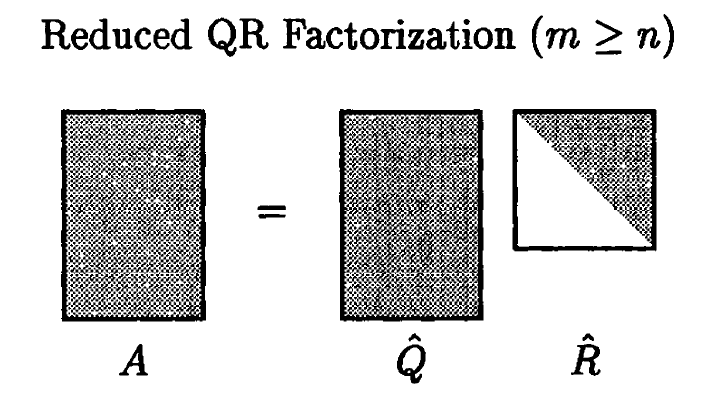
\includegraphics[width = 0.45\textwidth]{figs/TB_reducedQR}
%     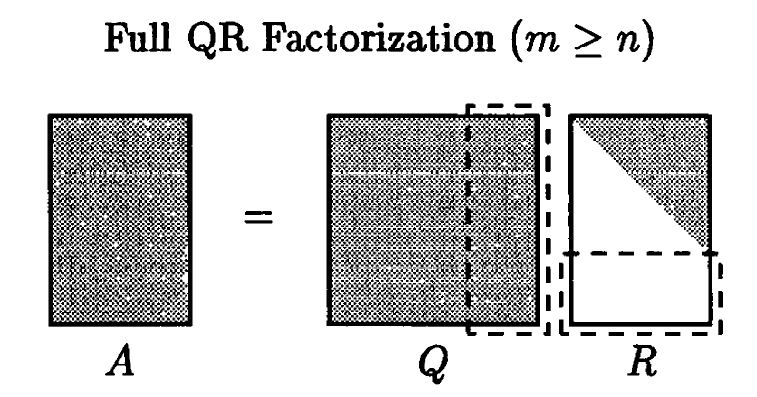
\includegraphics[width = 0.45\textwidth]{figs/TB_fullQR}
% \end{figure}

% \subsection{}
% We can interpret the formula for the solution of the least-squares problem
% \begin{align*}
%     \ve{\hat R} \ve x = \ve{\hat Q}^\top \ve b
% \end{align*}
% by using the full form of QR.

\section{Projectors}
A projector is a square matrix $\ve P$ that satisfies
\begin{align*}
    \ve P^2 = \ve P.
\end{align*}

\subsection{}
Assume $\ve P$ is a projector, and show that $\ve I-\ve P$ is also a projector.

\subsection{}
We can show that
\begin{align*}
    & \text{range}(\ve I-\ve P) = \text{null}(\ve P);\\
    & \text{null}(\ve I-\ve P) = \text{range}(\ve P);\\
    & \text{range}(\ve P) \cap \text{null}(\ve P) = 0.
\end{align*}

An orthogonal projector is a projector whose has the subspaces $\text{range}(\ve P)$ and $\text{null}(\ve P)$ orthogonal.

n.b.: An orthogonal projector $\ve P$ is not an orthogonal matrix! Why?

\subsection{}
Show that if $\ve P=\ve P^\top$ symmetric, the projector $\ve P$ is orthogonal (Hint: take one vector in $\text{range}(\ve P)$ and one in $\text{null}(\ve P)$, show that they must be orthogonal to each other). 

The reverse direction holds as well. Therefore the two definitions are equivalent.

\subsection{}
A special case of orthogonal projection is the projection onto a vector:
\begin{align*}
    \ve P_v = \frac{\ve v \ve v^\top}{\ve v^\top \ve v}.
\end{align*}
Show that it is indeed an orthogonal projector with range $\text{span}(\ve v)$.

\subsection{}
Another orthogonal projection is
\begin{align*}
    \ve P_{\perp v} = I-\frac{\ve v \ve v^\top}{\ve v^\top \ve v}.
\end{align*}
What is its null space? What is its range?

\section{Least squares and infections disease}
Let us assume an infectious disease with the following reported new
infections $I_i$ on each day $t_i$, for $i=1,\ldots,10$.
\begin{table}[h]\centering
  \caption{Number of new infections $I_i$ on days $t_i$.}
  \begin{tabular}{c||c|c|c|c|c|c|c|c|c|c|}
\hline
$t_i$: & 1 & 2 & 3 & 4 & 5 & 6 & 7 & 8 & 9 & 10\\ \hline
$I_i$: & 14 & 20 & 21 & 24 & 15 & 45 & 67 & 150 & 422 & 987\\ \hline
\end{tabular}
\end{table}
Using least squares fitting, we would like to understand the nature of
this growth. We consider two models to describe the connection between
time (i.e., days) $t$ and the number of new infections, both with 3
unknown parameters $(a,b,c)$:
\begin{equation*}%\label{poly}
  I(t) = a + b t + c t^2 \qquad \text{(polynomial model)}
\end{equation*}
\begin{equation*}%\label{exp}
  I(t) = a + bt + c\exp(t) \qquad \text{(exponential model)}
\end{equation*}
Our goal is to figure out which model describes the progression of the
infections better, and we use least squares fitting to figure that
out. Note that if a model would fit the data perfectly, $I(t_i) = I_i$
for all $i$. In general, you will not be able to find parameters that
satisfy this, and thus have to use least squares fitting (sometimes
this is also called \emph{regression}).

\subsection{} Formulate, assuming the polynomial model, the least squares
  problem for the parameters $\ve x=[a,b,c]^T$ by specifying the
  matrices $A$ and the vector $\ve b$:
  $$ \min_{\ve x\in \mathbb R^3}\|\ve A\ve x - \ve
  b \|_2^2
  $$

\subsection{}  Same as above, but for the exponential model.

\subsection{} Use a QR-factorization in MATLAB or Python to solve these
  problems and plot the data as points, as well as the model as a
  line. Repeat using the normal equations $\ve A^T\ve A\ve x =
  \ve A^T\ve b$.
\subsection{} To decide which model describes the data better, we need to
  compute the distance between the model and the data points. Take a
  look at the proof from class for how  the QR  factorization can be
  used to solve least squares  problems. In  particular, we found
  that:
  $$
  \|\ve A\ve x  - \ve  b\|_2^2 \ge \|\ve b_2\|_2^2,
  $$ where $\ve b_2 = \ve{\hat{\hat Q}}^\top\ve b$. We also
  found that this inequality is equality if $\ve x$ solves
  the least squares problem. Thus, the norm or $\ve b_2$ is a
  measure of how well the model fits the data. Use this to decide
  which of the two models above describes the data better.
  
    
    
\printbibliography

\end{document}